\documentclass[12pt, oneside]{amsart}
\usepackage[utf8]{inputenc}
\usepackage{geometry}
\geometry{verbose,tmargin=1.2in,bmargin=1.2in,lmargin=1.2in,rmargin=1.2in}
\usepackage{lmodern}
\usepackage{amsmath} 
\usepackage{amssymb}  
\usepackage[section]{placeins} 
\usepackage{bbm} 
\usepackage{amsthm}  
\usepackage{color} 
\usepackage[dvipsnames]{xcolor}
\linespread{2}  
\usepackage{booktabs} 
\usepackage{ragged2e}
\usepackage{lscape} 
\usepackage{colortbl}
\usepackage{tikz}
\usepackage{float}
\usepackage{morefloats}

\usepackage[hang, center]{subfigure}
\renewcommand{\thesubfigure}{\large \bf \Alph{subfigure}.}
\usepackage{graphicx}
\usepackage{soul}
\usepackage[countmax]{subfloat}
\usepackage{float}
\usepackage{rotfloat}
\usepackage{setspace}
\usepackage{esint}
\onehalfspacing
\usepackage[authoryear]{natbib}
\definecolor{MyDarkBlue}{rgb}{0,0.08,0.45}
\usepackage[unicode=true,pdfusetitle, bookmarks=true,bookmarksnumbered=false,bookmarksopen=false, breaklinks=false,pdfborder={0 0 1},colorlinks=true, linkcolor = MyDarkBlue, citecolor = MyDarkBlue, filecolor=MyDarkBlue, urlcolor=MyDarkBlue]{hyperref}
\usepackage{caption}
\usepackage{cleveref}
\usepackage[export]{adjustbox}

\PassOptionsToPackage{normalem}{ulem}
\usepackage{ulem}
 
\makeatletter

\numberwithin{equation}{section}

\DeclareMathOperator*{\plim}{plim}
\DeclareMathOperator*{\argmin}{argmin}
\DeclareMathOperator*{\argmax}{argmax}
\providecommand{\E}{\mathrm{E}}
\providecommand{\var}{\mathrm{var}}
\providecommand{\cov}{\mathrm{cov}}
\providecommand{\betahat}{\widehat{\beta}}

\makeatother

\title[Cash for Climate Adaptation]{Cash for Climate Adaptation in Uganda: \\
Experimental Design and Randomization$^{*}$}

\author{ $^{\ddagger}$}
\author{ $^{\mp}$}
\author{ $^{\dagger}$}

\thanks{$^{*}$Acknowledgments.}
\thanks{$^{\ddagger}$Affiliation. E-mail: \texttt{}.}
\thanks{$^{\mp}$Affiliation. E-mail: \texttt{}.}
\thanks{$^{\dagger}$Affiliation. E-mail: \texttt{}.}

\begin{document}

\maketitle
\begin{center}
This version: May 2026
\end{center}

\bigskip

\begin{abstract}
[Abstract placeholder.]
\end{abstract} 

\vfill
\thispagestyle{empty}
\newpage
\setcounter{page}{1}
\doublespacing

%% ============================================================
\section{\label{sec_intro}Introduction}
%% ============================================================

[Introduction placeholder.]

%% ============================================================
\section{\label{sec_data}Data}
%% ============================================================

[Data placeholder.]

%% ============================================================
\section{\label{sec_emp}Empirical Strategy}
%% ============================================================

This section describes the experimental design, the construction of randomization clusters, and the power calculations that inform the study's ability to detect treatment effects.

%% ------------------------------------------------------------
\subsection{\label{sec_design}Experimental Design}
%% ------------------------------------------------------------

The program is implemented across 134 settlements in Bulambuli and Amuria Districts, Uganda, reaching approximately 11,801 recipients. All eligible adults in selected settlements receive a \$644 USD lump-sum cash transfer (\$50 token followed by \$594 lump sum). Of these, 119 settlements have confirmed GPS coordinates and are included in the randomization; 15 settlements in Bulambuli are pending field collection of coordinates. Settlements in Amuria are substantially larger than those in Bulambuli: using parish-level population data from the Uganda Bureau of Statistics (UBOS-NPHC 2024), we estimate that Amuria settlements average approximately 222 households, while Bulambuli settlements average approximately 29 households---a ratio of nearly 8:1. Despite having only 16 settlements, Amuria accounts for roughly half of the program's total households (3,558 of 6,928).

The evaluation uses a three-arm design with randomization at the cluster level (see Section \ref{sec_clusters} for cluster construction):

\begin{itemize}
    \item \textbf{Group 1}: Standard Large Lump Sum (LLS) program with a default ``Community Empowerment'' Baraza. Cash delivered early in the rollout (June--November 2026). Serves as control for the plus comparison and as treatment for the cash comparison.
    \item \textbf{Group 2}: Same cash transfer and timeline as Group 1, but with a modified Baraza framing transfers as supporting climate adaptation, plus household-level randomized components (historical climate information and adaptation aspirations planning).
    \item \textbf{Group 3}: Standard LLS with default Baraza, delivered later in the rollout. Serves as control for the cash comparison.
\end{itemize}

The design addresses two causal questions. First, what is the effect of unconditional cash transfers on climate-adaptive behaviors (Group 1 vs.\ Group 3)? Second, what is the additional effect of climate-focused ``plus'' components (Group 2 vs.\ Group 1)?

%% ------------------------------------------------------------
\subsection{\label{sec_hypotheses}Hypotheses and Estimation Equations}
%% ------------------------------------------------------------

The design addresses three questions, each with a distinct estimation equation.

\paragraph{Question 1: Cash effect (Group 1 vs.\ Group 3).}

\begin{equation}
Y_{iv} = \alpha + \beta D_v^{(1)} + \gamma Y_{iv,\text{baseline}} + \delta X_{iv} + \varepsilon_{iv}
\end{equation}

\noindent where $Y_{iv}$ is the outcome for household $i$ in village $v$ at follow-up (e.g., 3-month livelihood investment), $D_v^{(1)} = 1$ if the village is in Group 1 (early cash) and 0 if in Group 3 (late cash), $Y_{iv,\text{baseline}}$ is the same outcome measured at baseline, and $X_{iv}$ are household characteristics. We cluster standard errors at the village level and do not include village fixed effects because treatment is assigned at the village level. Power comes from the number of clusters (16 per arm).

\paragraph{Question 2: Baraza framing effect (Group 1 vs.\ Group 2c).}

\begin{equation}
Y_{iv} = \alpha + \beta D_v^{(2c)} + \gamma Y_{iv,\text{baseline}} + \delta X_{iv} + \varepsilon_{iv}
\end{equation}

\noindent We cluster standard errors at the village level and do not include village fixed effects because Baraza type varies at the village level and fixed effects would absorb that variation. This comparison has fewer clusters than Q1 (16 vs.\ 7 clusters).

\paragraph{Question 3: Plus components (Group 2a vs.\ Group 2b vs.\ Group 2c).}

\begin{equation}
Y_{iv} = \alpha + \beta D_{i}^{(2a)} + \gamma Y_{iv,\text{baseline}} + \delta X_{iv} + \mu_v + \varepsilon_{iv}
\end{equation}

\noindent We include village fixed effects $\mu_v$ because randomization is at the household level within villages. Standard errors are clustered at the village level. Power comes from the number of households ($\sim$313 per sub-arm), allowing detection of effects of $\sim$0.19 SD.

%% ------------------------------------------------------------
\subsection{\label{sec_clusters}Cluster Construction and Randomization}
%% ------------------------------------------------------------

The two study districts are geographically separated by approximately 98 kilometers, eliminating any concern about cross-district spillovers (see Figure \ref{fig:villages_all} in the Appendix for a map of all 134 settlements by district). Figure \ref{fig:villages_size} displays settlement locations with dot size proportional to estimated households, illustrating the stark size asymmetry between districts. The two districts are approximately 98 km apart.

\begin{figure}[H]
\centering
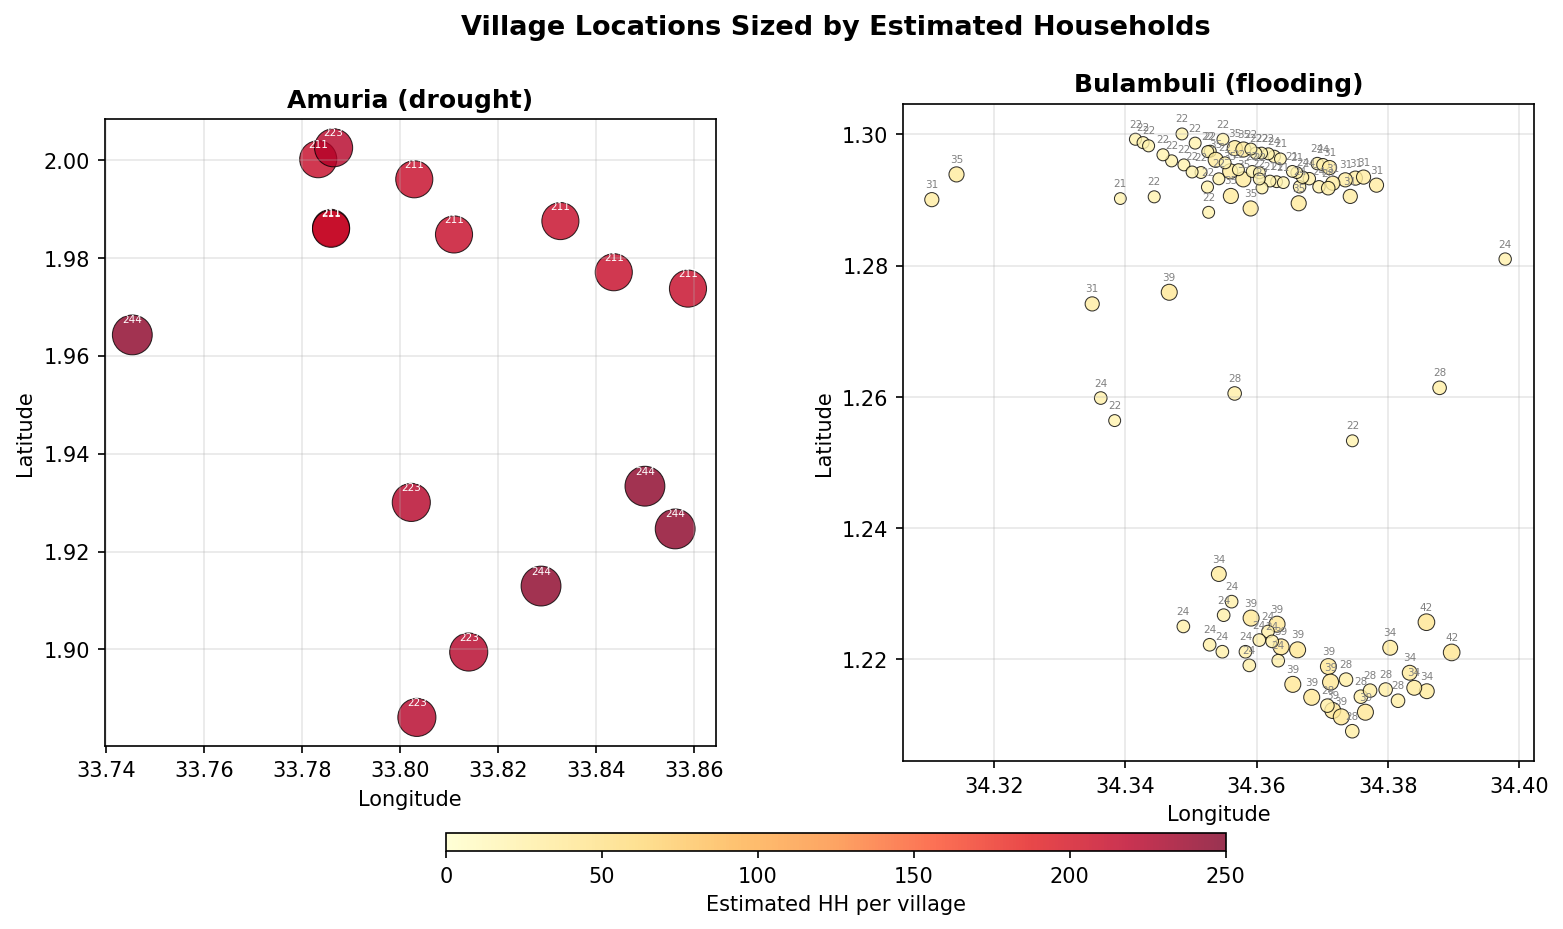
\includegraphics[width=0.95\textwidth]{figures/villages_by_size.png}
\caption{Settlement locations sized by estimated households per settlement (UBOS 2024 parish-level data). The two districts are approximately 98 km apart.}
\label{fig:villages_size}
\end{figure}

\subsubsection{Geographic Clustering}

To mitigate spillovers between neighboring settlements, we construct randomization clusters using hierarchical agglomerative clustering (complete linkage) on settlement GPS coordinates. Under complete linkage, two settlements are merged into the same cluster only if the maximum pairwise distance between any two settlements in the resulting cluster is below the distance threshold. We evaluate thresholds of 1, 2, and 3 kilometers.

Figure \ref{fig:cluster_distance} shows how the number of clusters varies with the distance threshold. Bulambuli settlements collapse rapidly from 46 clusters at 0.5 km to 8 clusters at 3 km, reflecting their geographic density. Amuria settlements remain relatively stable at 9--14 clusters, reflecting their natural spatial separation. Appendix Figures \ref{fig:geo_1km}--\ref{fig:geo_3km} display the resulting randomization under geographic clustering at each threshold.

\begin{figure}[H]
\centering
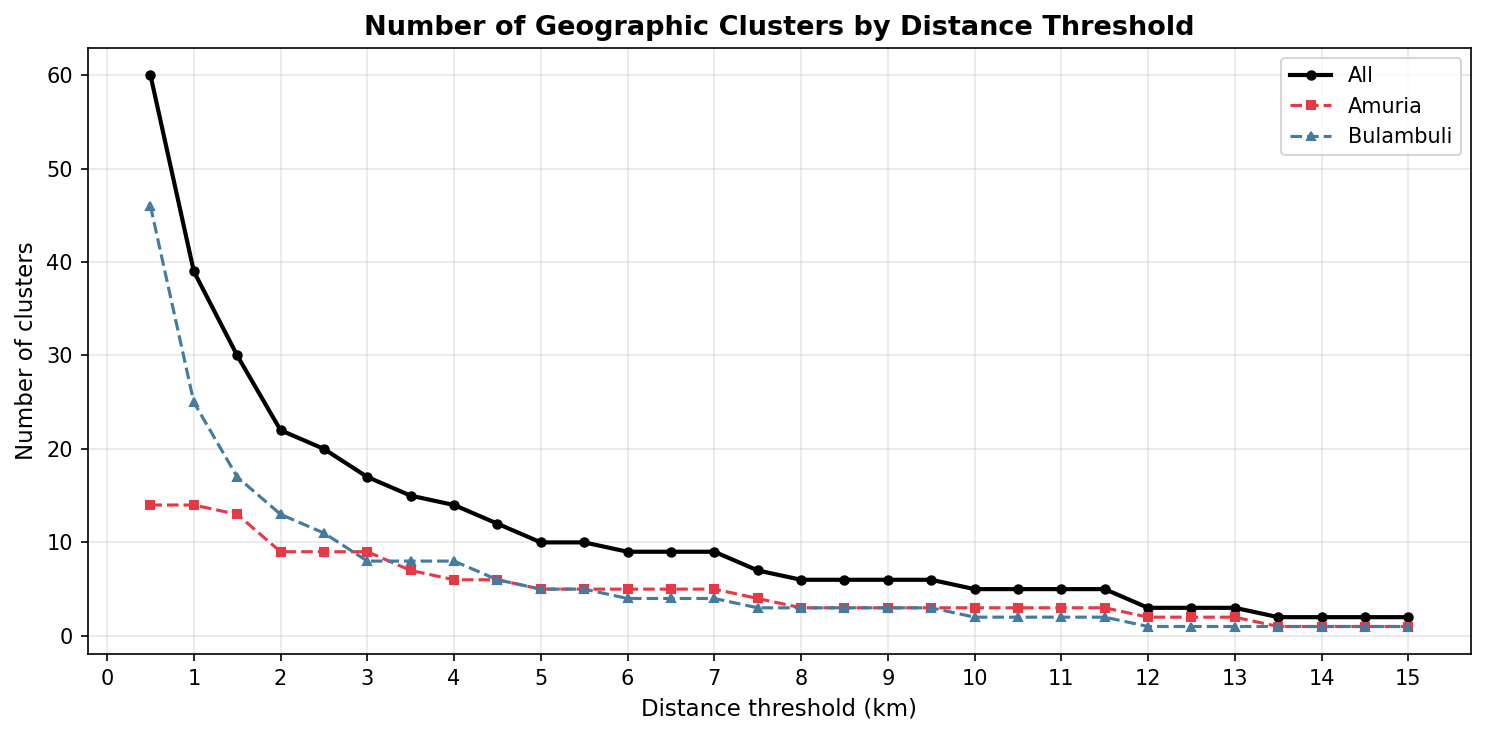
\includegraphics[width=0.95\textwidth]{figures/clusters_by_distance.png}
\caption{Number of geographic clusters as a function of the distance threshold.}
\label{fig:cluster_distance}
\end{figure}

We adopt the 1 km threshold, which yields 39 clusters (14 in Amuria, 25 in Bulambuli). This threshold balances two competing objectives: minimizing spillover contamination between arms and maximizing the number of randomization units for statistical power.

\subsubsection{The Spillover Problem}

A naive village-level randomization assigns each of the 134 settlements independently to one of the three arms. While this maximizes the number of randomization units (and thus statistical power), it creates a severe spillover problem in Bulambuli, where settlements are densely packed within 1--2 kilometers of each other. Figure \ref{fig:village_random} illustrates a simulated village-level randomization: neighboring settlements in Bulambuli are assigned to different arms, meaning that recipients in early-cash settlements and delayed-cash settlements share local markets, trade networks, and social ties. Treatment effects from cash settlements would contaminate control settlements, biasing the estimated cash effect toward zero.

\begin{figure}[H]
\centering
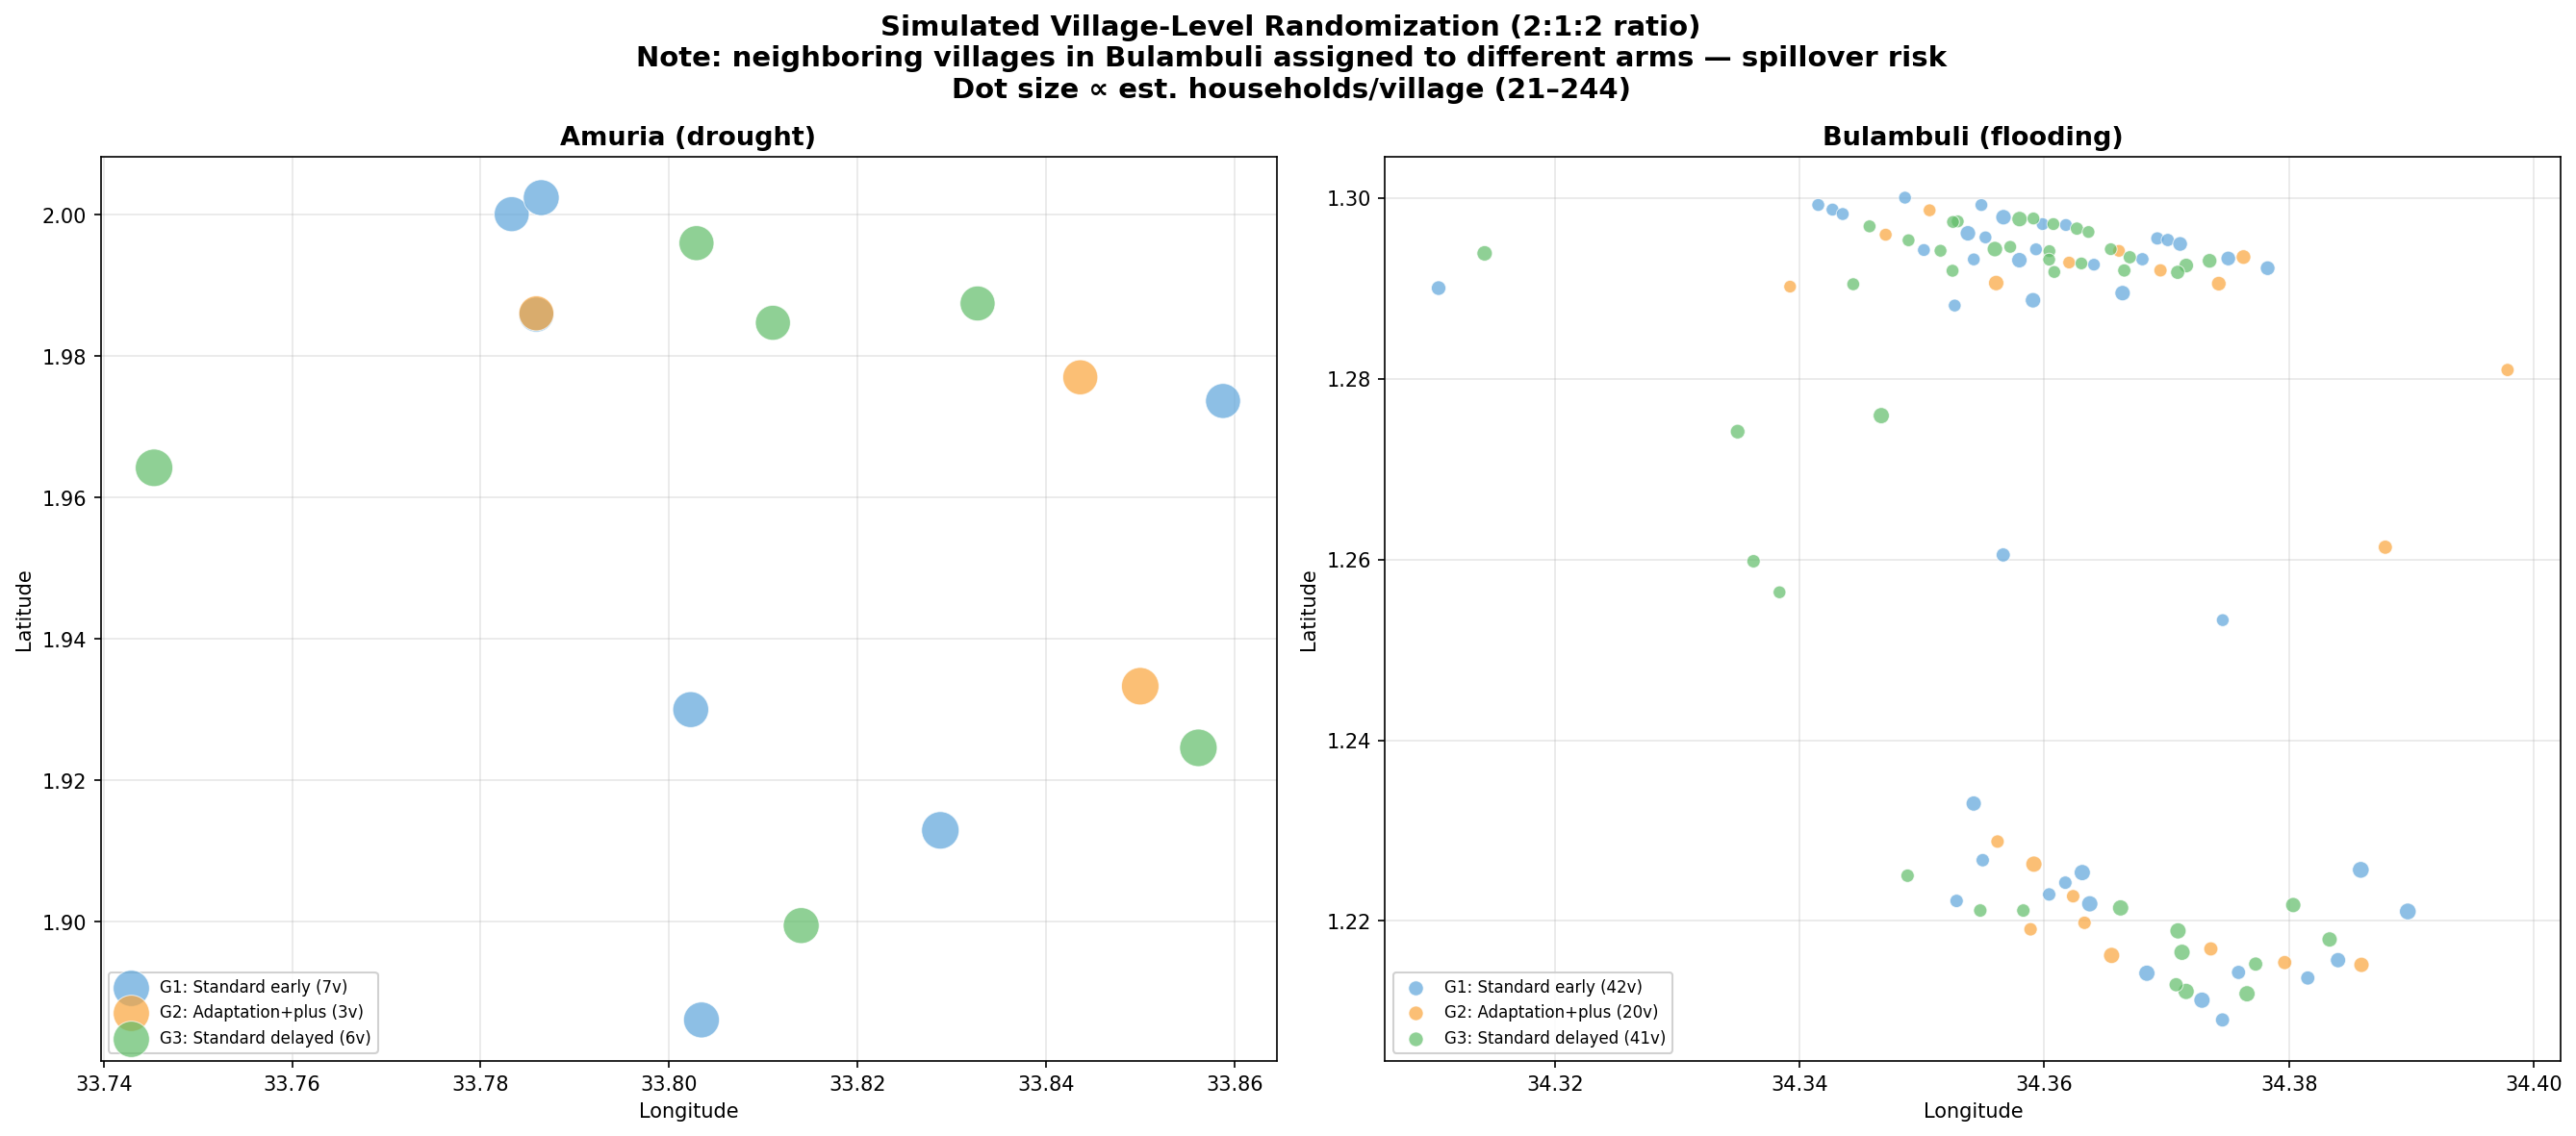
\includegraphics[width=0.95\textwidth]{figures/randomization_village_level.png}
\caption{Simulated village-level randomization (2:1:2 ratio). Note the extensive mixing of arms among neighboring villages in Bulambuli.}
\label{fig:village_random}
\end{figure}

\subsubsection{Cluster Assignment}

Figure \ref{fig:clusters_final} displays the 39 geographic clusters at the 1 km threshold. Cluster sizes range from 1 to 13 villages (median 2). In Amuria, most clusters contain a single village due to the natural spatial separation between settlements. In Bulambuli, the dense settlement pattern produces several large clusters, particularly in the northern parishes. Fifteen villages with missing GPS coordinates (all in Bulambuli) are excluded from the clustering and randomization pending field collection of coordinates (see Appendix Figure \ref{fig:clusters_22} for the earlier 22-cluster design at 3 km that was superseded by this approach).

\begin{figure}[H]
\centering
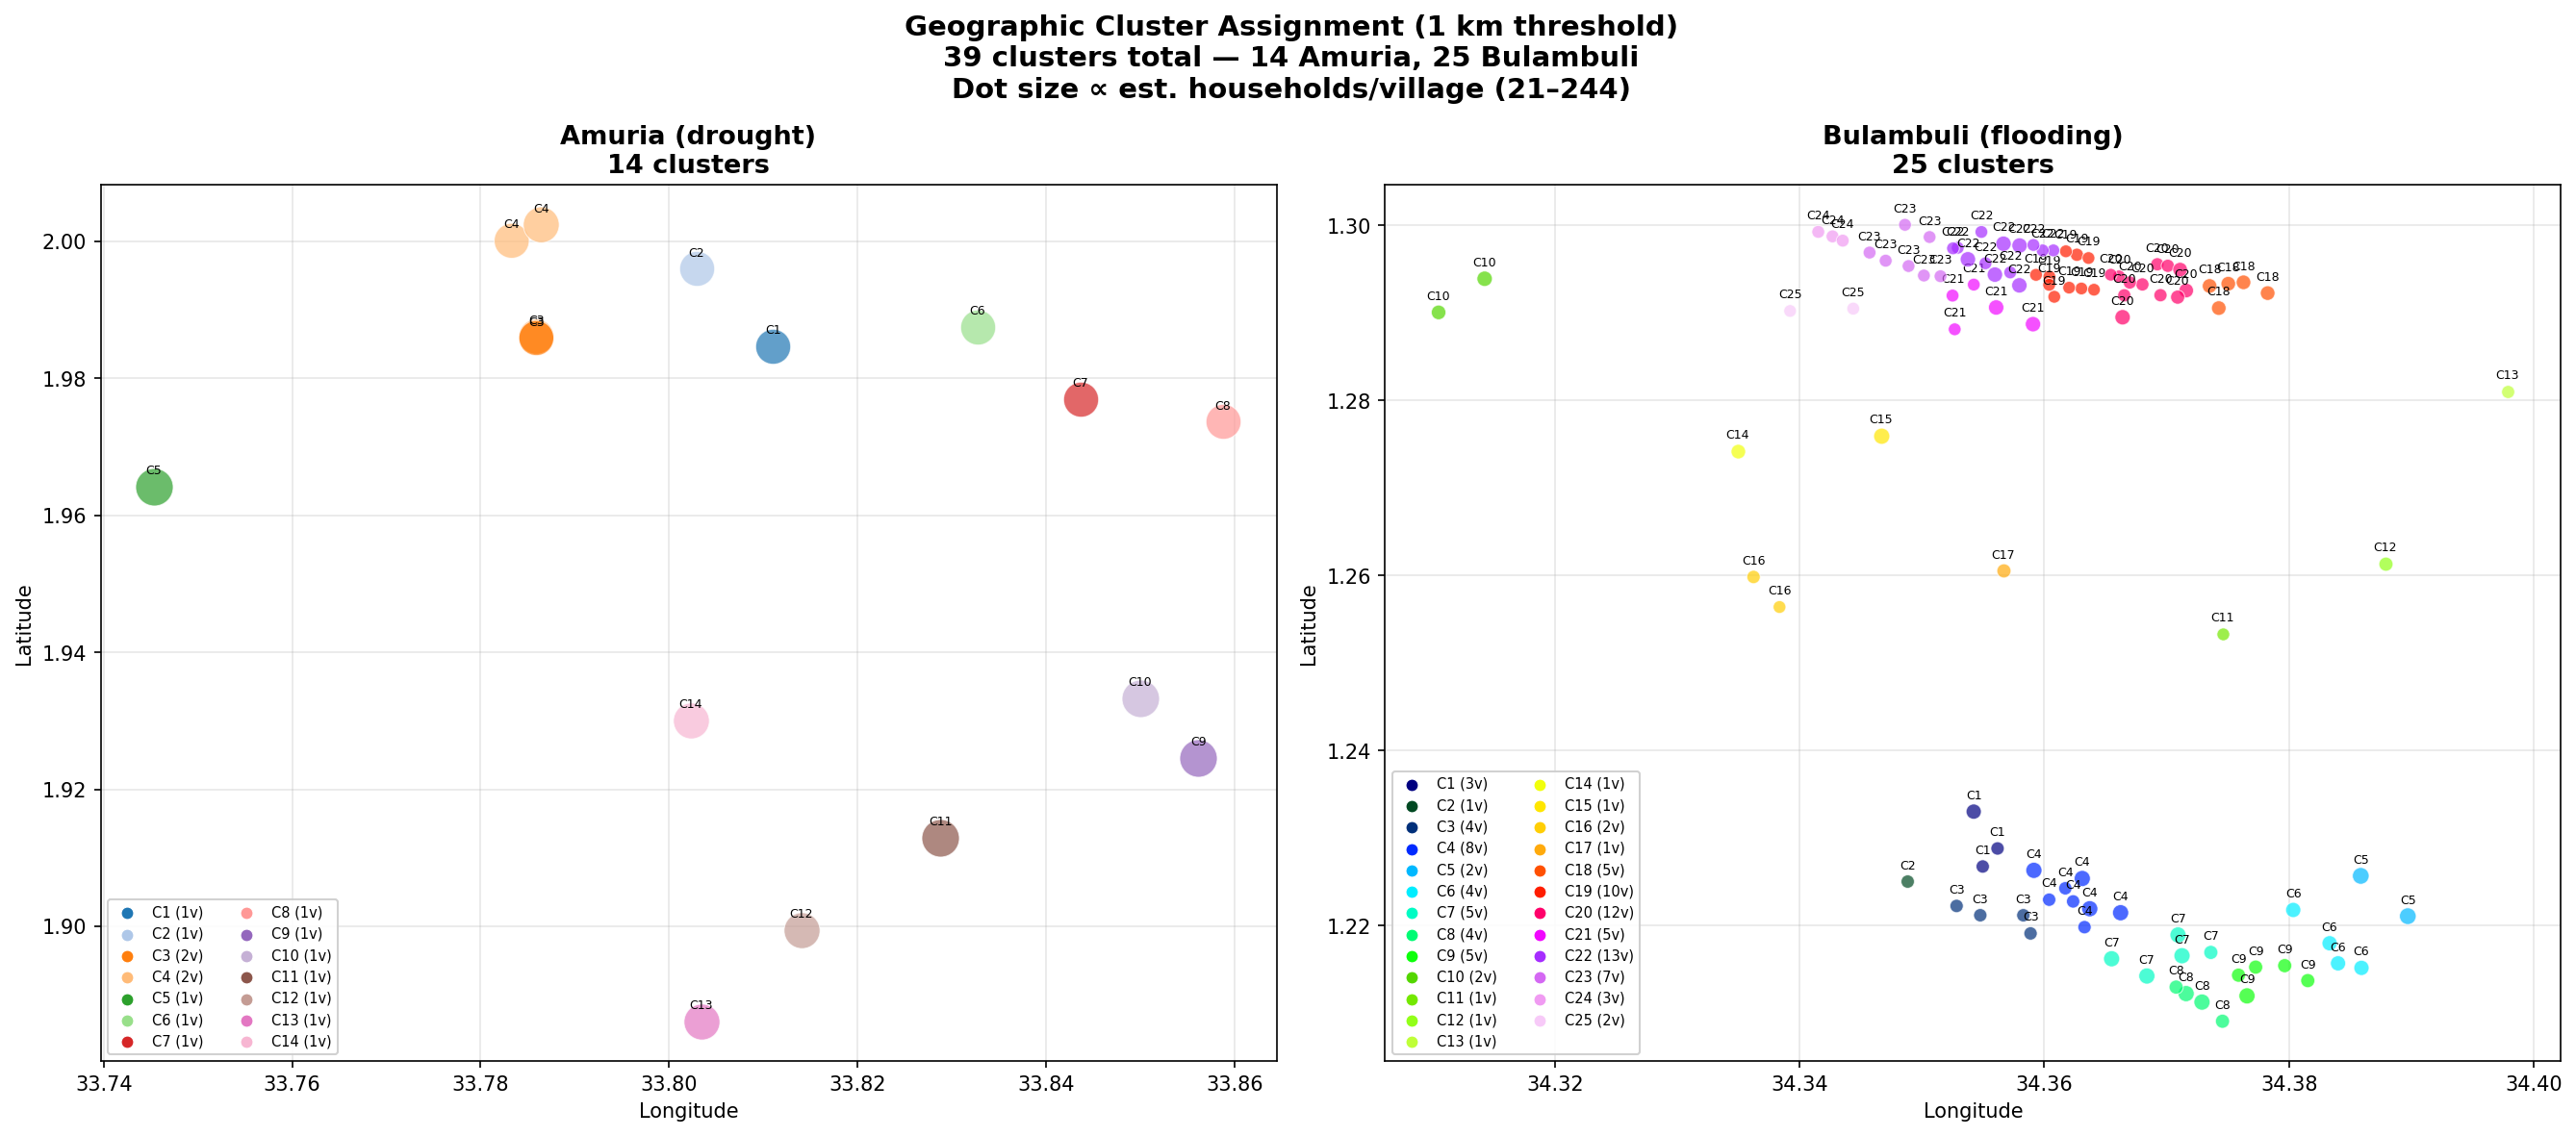
\includegraphics[width=0.95\textwidth]{figures/geo_clusters_1km_39.png}
\caption{Geographic cluster assignment: 39 clusters at 1 km threshold (14 Amuria, 25 Bulambuli). Dot size proportional to estimated households per village.}
\label{fig:clusters_final}
\end{figure}

\subsubsection{Randomization}

We randomize the 39 clusters into three arms using a 2:1:2 allocation ratio, stratified by district. Groups 1 and 3 receive more clusters to maximize power for the primary comparison (Q1: cash effect), while Group 2 receives fewer clusters because its main identification (Q3: plus components) relies on household-level randomization within villages. The randomization is performed once with a fixed seed (seed $= 2026$) and documented for reproducibility. Figure \ref{fig:randomization_final} displays the resulting assignment.

\begin{figure}[H]
\centering
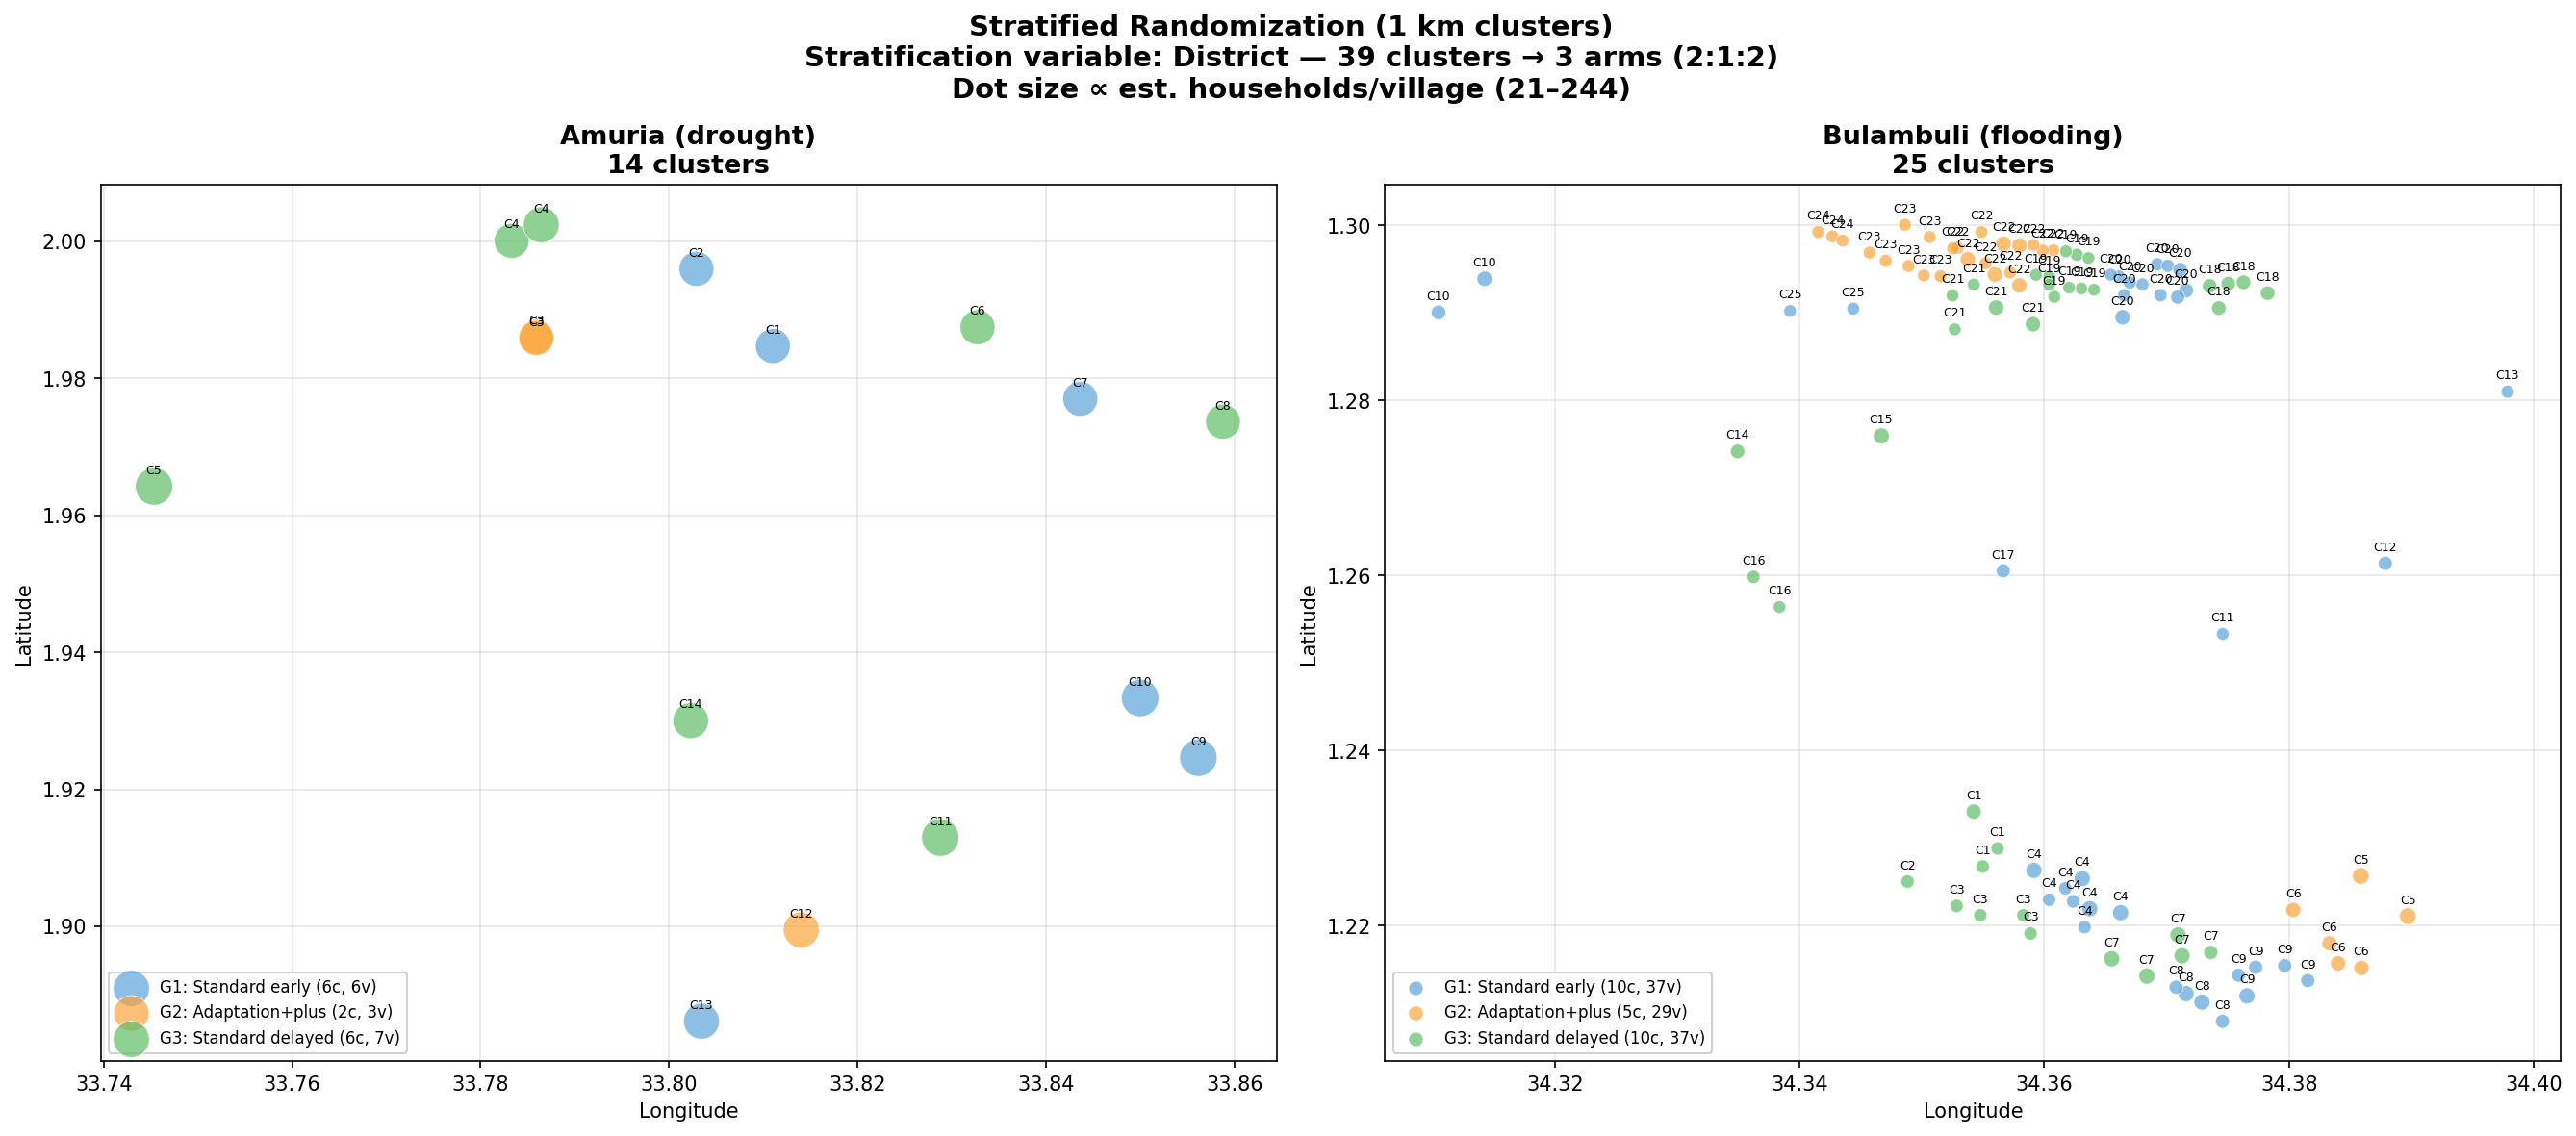
\includegraphics[width=0.95\textwidth]{figures/randomization_1km_39.png}
\caption{Final randomization of 39 clusters into three arms (2:1:2 ratio, stratified by district).}
\label{fig:randomization_final}
\end{figure}

\noindent Table \ref{tab:randomization} summarizes the allocation:

\begin{table}[H]
\centering
\small
\caption{Randomization summary: clusters and villages by arm and district}
\label{tab:randomization}
\begin{tabular}{lcccc}
\toprule
 & G1: Standard early & G2: Adaptation+plus & G3: Standard delayed & Total \\
\midrule
Amuria   & 6c, 6v  & 2c, 3v  & 6c, 7v  & 14c, 16v \\
Bulambuli & 10c, 37v & 5c, 29v & 10c, 37v & 25c, 103v \\
\midrule
\textbf{Total} & \textbf{16c, 43v} & \textbf{7c, 32v} & \textbf{16c, 44v} & \textbf{39c, 119v} \\
\bottomrule
\multicolumn{5}{l}{\footnotesize \textit{Note:} c = clusters, v = villages. For example, 6c, 6v = 6 clusters containing 6 villages.} \\
\end{tabular}
\end{table}

%% ------------------------------------------------------------
\subsection{\label{sec_power}Power Calculations}
%% ------------------------------------------------------------

We evaluate the minimum detectable effect (MDE) for the primary comparison (Q1: cash vs.\ no cash, Group 1 vs.\ Group 3) under the cluster-randomized design. The MDE depends on the number of clusters per arm, the number of households surveyed per cluster, the intra-cluster correlation coefficient (ICC), and the baseline-endline correlation from the panel design.

\subsubsection{Parameters}

We draw on two literature reviews to calibrate the power calculations (see Appendix \ref{sec_appendix_params} for full details). For the ICC, a synthesis of empirical estimates from cash transfer evaluations in East Africa---including \citet{haushofer2016short}, \citet{mcintosh2022cash}, \citet{egger2022general}, and \citet{aggarwal2023}---yields a recommended range of 0.05 (low), 0.10 (medium), and 0.15 (high) for livelihood investment outcomes. The most directly relevant Uganda estimate is ICC $= 0.07$ from \citet{icancar2025}. For baseline outcome parameters, we use a central estimate of 75,000 UGX per month for livelihood investment spending (SD $= 112{,}500$ UGX), calibrated to extreme-poor populations in Eastern Uganda using the SAGE evaluation \citep{sage2012} and \citet{blattman2014}. For the binary diversification outcome, we assume a baseline rate of 20\%, informed by non-agricultural participation rates in \citet{aggarwal2023} and \citet{mcintosh2022cash}.

The panel design (baseline and endline surveys of the same households) provides an ANCOVA gain through the baseline-endline correlation, which we set at $\rho = 0.5$. We survey 30\% of households per settlement, yielding a weighted average of approximately 29 households surveyed per cluster (reflecting the mix of large Amuria settlements and small Bulambuli settlements).

\subsubsection{Minimum Detectable Effects}

Figure \ref{fig:power} displays the MDE as a function of the number of clusters per arm, for both the continuous outcome (livelihood investment, left panel) and the binary outcome (income diversification, right panel). Horizontal reference lines indicate effect sizes observed in prior GiveDirectly evaluations. The blue shaded region marks our cluster-based design (16 clusters per arm).

\begin{figure}[H]
\centering
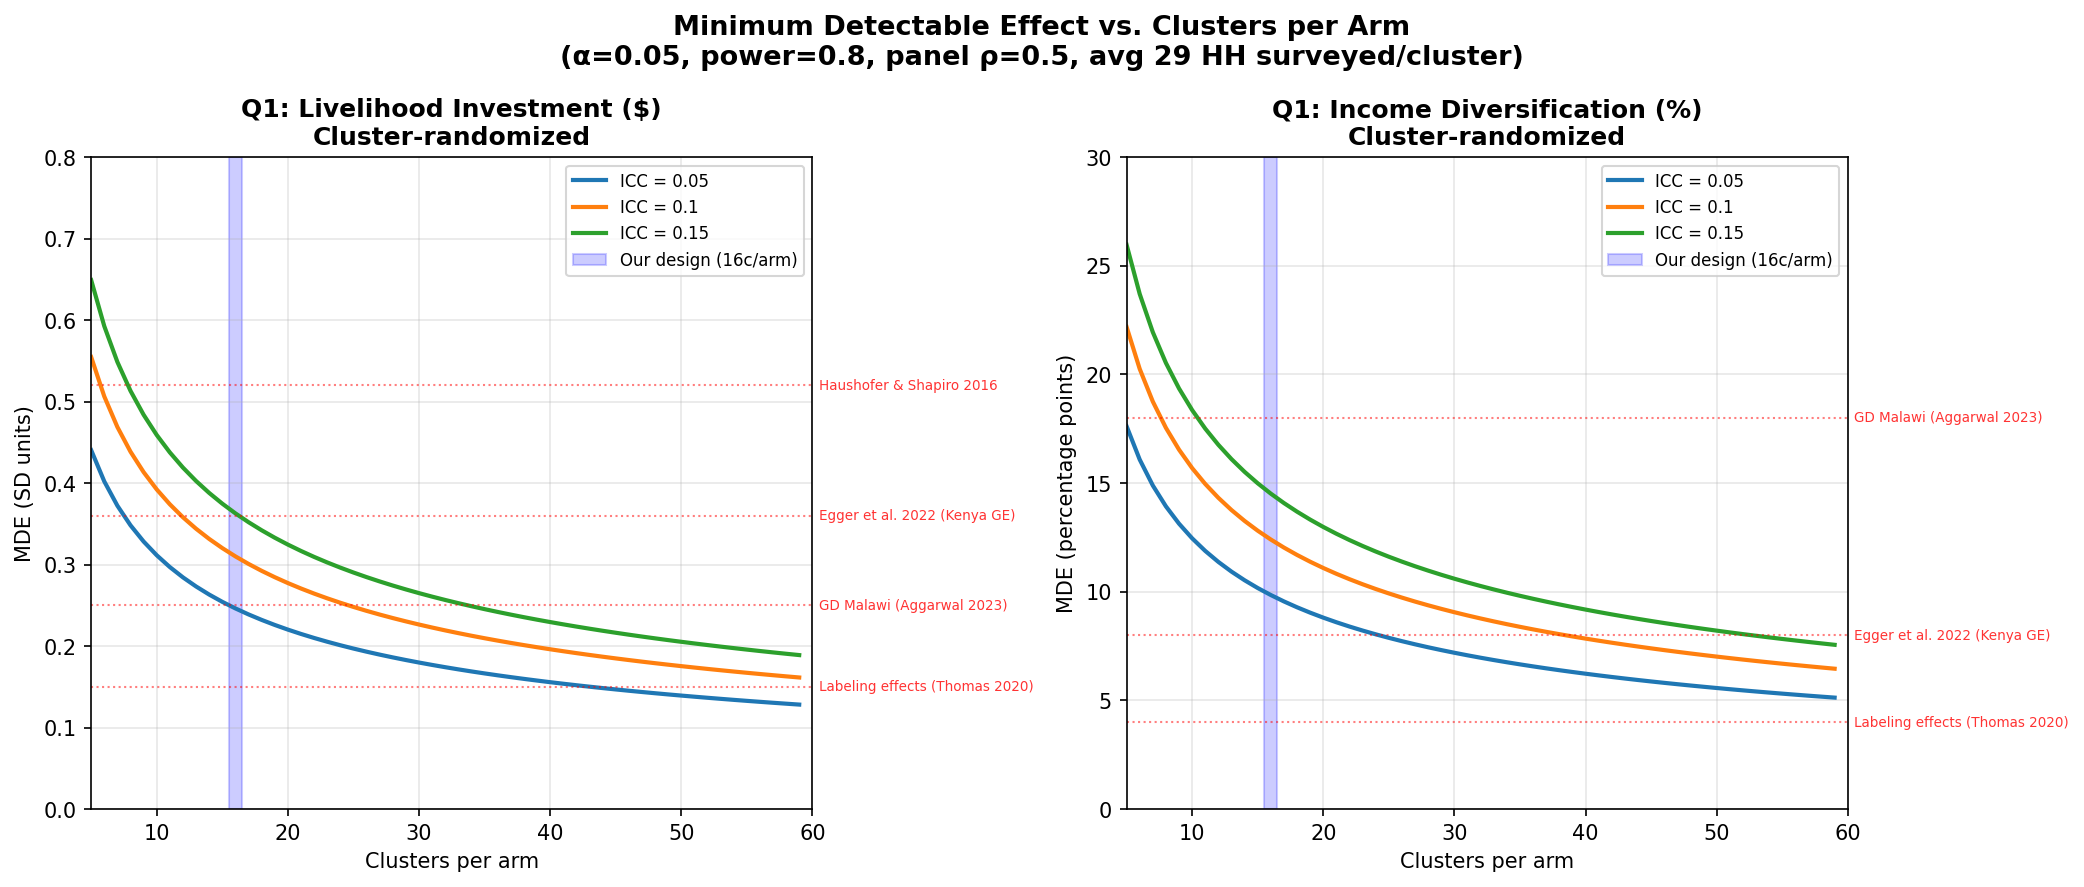
\includegraphics[width=0.95\textwidth]{figures/power_mde_vs_clusters.png}
\caption{Minimum detectable effect vs.\ number of clusters per arm. Blue region: our 39-cluster design (16 per arm). Horizontal lines: effect sizes from prior cash transfer evaluations.}
\label{fig:power}
\end{figure}

At 16 clusters per arm, the MDE ranges from 0.25 to 0.36 SD for the continuous outcome, within the range of 0.25--0.52 SD effects observed in prior GiveDirectly programs \citep{haushofer2016short, egger2022general}. For the binary diversification outcome, the design can detect changes of approximately 10--15 percentage points. The GiveDirectly Malawi program observed an 18 percentage point increase in business ownership \citep{aggarwal2023}, suggesting that effects of this magnitude would be detectable.

For Q2 (baraza framing), the comparison between Group 1 (16 clusters) and Group 2 (7 clusters) yields MDEs of 0.37--0.55 SD for the continuous outcome. Given that labeling and messaging effects in the literature are typically 0.10--0.25 SD \citep{thomas2020}, Q2 is likely underpowered for small effects and should be interpreted as exploratory.

For Q3 (plus components), randomization is at the household level within Group 2 settlements. With approximately 313 households per sub-arm, the MDE is 0.19 SD for the continuous outcome and 7.8 percentage points for the binary outcome.

%% ============================================================
\newpage
\appendix
\section{\label{sec_appendix}Appendix: Program Design Details}
%% ============================================================

\subsection{Program Overview}

The Quadrature Climate Foundation (QCF) funds a program with GiveDirectly to test whether unconditional cash transfers can support climate adaptation in Uganda. The program targets 11,801 recipients across 134 settlements in Bulambuli District (flooding, waterlogging) and Amuria District (drought). Each recipient receives \$644 USD in two tranches: a \$50 token transfer after enrollment, followed by a \$594 lump sum several weeks later.

\subsection{Theory of Change}

Cash relaxes liquidity and capital constraints, enabling households to make forward-looking livelihood investments that support ex-ante climate adaptation. Households may allocate transfers toward: (1) expanding existing livelihoods, (2) diversifying into new income-generating activities, (3) making existing livelihoods more resilient to climate risk, (4) general consumer durables, or (5) climate-protective durable assets. Channels (1), (2), and (4) correspond to the standard LLS economic pathway; channels (3) and (5) correspond to the climate adaptation pathway.

\subsection{Indicators}

The evaluation collects 15 standard LLS indicators (food expenditure, household consumables, education, consumer durables, savings/debt, livelihood investments, healthcare, food insecurity, dietary diversity, psychological well-being, income-generating activity, hours worked, asset ownership, and debt/savings) and 10 non-standard climate adaptation indicators organized into four domains:

\begin{enumerate}
    \item \textbf{Expectations and Constraints:} Perceived ability to prepare for climate risks; priority support needed for adaptation.
    \item \textbf{Allocation Choices:} Livelihood investment decomposed into expansion, diversification, and resilience categories.
    \item \textbf{Structural Adjustment:} Climate-related occupational change; climate-related migration.
    \item \textbf{Spillovers and System Effects:} Individual investments with community spillovers; positive coping in response to shock; maladaptive coping behavior.
\end{enumerate}

\subsection{M\&E Design}

Surveys are administered to 30\% of recipients ($\sim$3,540 households) at baseline and endline, using a panel design. Baseline data collection occurs at enrollment before the first transfer. Endline occurs approximately three months after the final transfer delivery. Surveys are conducted in person and take approximately 30 minutes.

\subsection{Limitations}

\begin{enumerate}
    \item No direct shock tracking between baseline and endline.
    \item No non-recipient comparison group for the within-group analysis; the staggered design (Group 1 vs.\ Group 3) provides the cash comparison.
    \item Limited cross-program comparability.
    \item Baraza labeling is integrated into the program design and is not separately estimated.
\end{enumerate}

%% ============================================================
\section{\label{sec_appendix_melp}Appendix: MELP Key Information}
%% ============================================================

The research questions and three-arm design are described in Sections \ref{sec_design} and \ref{sec_hypotheses}.

\subsection{M\&E Survey Design}

\begin{itemize}
    \item 30\% of recipients surveyed at baseline and endline ($\sim$3,540 households).
    \item Panel design: same households at both waves.
    \item Baseline at enrollment (before first transfer); endline $\sim$3 months after final transfer.
    \item In-person surveys, $\sim$30 minutes.
\end{itemize}

\subsection{Standard LLS Indicators (1--15)}

\begin{enumerate}
    \item Spend on food
    \item Spend on household consumables
    \item Spend on children's education
    \item Spend on consumer durables
    \item Save or repay debt
    \item Spend on livelihood investments
    \item Spend on healthcare
    \item \% experiencing moderate/severe food insecurity
    \item \% consuming $\geq$5 food groups
    \item Psychological well-being score
    \item \% engaged in income-generating activities
    \item Average hours worked per week
    \item \% reporting increased income-generating activity
    \item \% owning productive/non-productive assets
    \item Total value of debt and savings
\end{enumerate}

\subsection{Non-Standard Climate Adaptation Indicators}

\textbf{0. Experienced Climate Shock} --- \% reporting a climate-related shock and timing.

\medskip
\noindent\textbf{I. Expectations \& Constraints}
\begin{enumerate}
    \item Perceived ability to prepare for climate risks
    \item Priority support needed for climate adaptation
\end{enumerate}

\noindent\textbf{II. Allocation Choices}
\begin{enumerate}
    \setcounter{enumi}{2}
    \item Livelihood investment --- expansion (continuing pre-existing activities)
    \item Livelihood investment --- diversification (new income-generating activities)
    \item Livelihood investment --- resilience (protective improvements to existing livelihoods)
\end{enumerate}

\noindent\textbf{III. Structural Adjustment}
\begin{enumerate}
    \setcounter{enumi}{5}
    \item Climate-related occupational change
    \item Climate-related migration
\end{enumerate}

\noindent\textbf{IV. Spillovers \& System Effects}
\begin{enumerate}
    \setcounter{enumi}{7}
    \item Individual investments with community spillovers
    \item Positive coping in response to shock
    \item Maladaptive coping behavior (charcoal burning, bush burning, wetland encroachment)
\end{enumerate}

\subsection{Reporting Timeline}

\begin{itemize}
    \item First report: October 2026
    \item Final report: October 2027
\end{itemize}

%% ============================================================
\section{\label{sec_appendix_params}Appendix: Power Calculation Parameters}
%% ============================================================

This appendix documents the empirical sources for the ICC values and baseline outcome parameters used in the power calculations (Section \ref{sec_power}). M\&E surveys are administered to 30\% of recipients in each settlement, yielding the household counts per cluster used throughout.

\subsection{Intra-Cluster Correlation Coefficients}

The ICC determines the proportion of total outcome variance attributable to between-cluster differences. Table \ref{tab:icc} summarizes empirical estimates from cash transfer evaluations and household surveys in rural Sub-Saharan Africa.

\begin{table}[H]
\centering
\small
\caption{Empirical ICC estimates from rural Sub-Saharan Africa}
\label{tab:icc}
\begin{tabular}{llcll}
\toprule
Domain & Outcome & ICC & Type & Source \\
\midrule
Consumption & Total consumption & 0.25 & Reported & World Bank (2019) \\
Consumption & Food expenditure & 0.16 & Reported & World Bank (2019) \\
Consumption & Monthly expenditure & 0.06 & Derived & Haushofer \& Shapiro (2016) \\
Consumption & Monthly expenditure & 0.05 & Derived & McIntosh \& Zeitlin (2022) \\
Consumption & Annual expenditure & 0.07 & Derived & ICAN-ICAR (2025), Uganda \\
\midrule
Food security & Dietary diversity & 0.03 & Derived & McIntosh \& Zeitlin (2022) \\
Food security & Not worried about food & 0.02 & Derived & Psychology of Poverty (2021) \\
Food security & Food security index & 0.04 & Derived & Haushofer \& Shapiro (2016) \\
\midrule
Livelihood & Livestock (TLU) & 0.12 & Derived & Psychology of Poverty (2021) \\
Livelihood & Irrigation adoption & 0.18 & Reported & Asian J. Agric. Ext. (2025) \\
Livelihood & Business entry & 0.07 & Derived & McIntosh \& Zeitlin (2022) \\
\midrule
Assets & Non-land asset index & 0.11 & Derived & Haushofer \& Shapiro (2016) \\
Assets & Productive asset value & 0.09 & Derived & McIntosh \& Zeitlin (2022) \\
\midrule
Income & Non-agricultural income & 0.06 & Derived & Aggarwal et al. (2023) \\
Income & Enterprise revenue & 0.10 & Reported & Egger et al. (2022) \\
Income & Wage labor participation & 0.05 & Derived & McIntosh \& Zeitlin (2022) \\
\bottomrule
\end{tabular}
\end{table}

Based on this synthesis, we adopt the following ranges: 0.05--0.15 for livelihood investment and income diversification (primary outcomes), and 0.01--0.05 for food security (secondary). The most directly relevant Uganda estimate is ICC $= 0.07$ from ICAN-ICAR (2025).

\citet{egger2022general} document substantial spatial interference in the GiveDirectly Kenya trial, where treatment in one village affected enterprise outcomes in neighboring untreated villages. This motivates our geographic clustering approach (Section \ref{sec_clusters}).

\subsection{Baseline Outcome Means and Standard Deviations}

Table \ref{tab:baseline} summarizes baseline estimates from national surveys and experimental evaluations, prioritizing extreme-poor populations in Eastern Uganda and comparable settings.

\begin{table}[H]
\centering
\small
\caption{Empirical baseline means and standard deviations}
\label{tab:baseline}
\begin{tabular}{llrrll}
\toprule
Domain & Variable & Mean & SD & Setting & Source \\
\midrule
Consumption & HH monthly exp. (UGX) & 372,128 & 154,611 & Uganda (rural) & UNHS 2019/20 \\
Consumption & HH monthly cons. (UGX) & 40,599 & 16,867 & Uganda (extreme poor) & SAGE 2012 \\
Consumption & HH monthly cons. (USD PPP) & 158 & 296 & Kenya (rural) & Haushofer (2016) \\
\midrule
Livelihood & Monthly earnings (USD) & 20 & 34 & Uganda (north) & Blattman (2014) \\
Livelihood & Non-ag income (USD PPP) & 15.28 & 18.10 & Malawi (rural) & Aggarwal (2023) \\
Livelihood & HH revenue (USD PPP) & 49 & 85 & Kenya (rural) & Haushofer (2016) \\
\midrule
Food security & Severe food insecurity (\%) & 60.2 & 0.49 & Uganda (eastern) & Cambridge (2024) \\
Food security & Not worried about food (\%) & 15.0 & 0.36 & Malawi (rural) & Psych. Poverty (2021) \\
\midrule
Assets & Non-land assets (USD PPP) & 495 & 580 & Kenya (rural) & Haushofer (2016) \\
Assets & Livestock value (USD PPP) & 127 & 230 & Kenya (rural) & Haushofer (2016) \\
\bottomrule
\end{tabular}
\end{table}

Our target population (85\% multidimensionally poor in Bulambuli) is closer to the SAGE extreme-poor sample than to the Kenya GiveDirectly or national Uganda averages. We adopt a central estimate of 75,000 UGX/month for livelihood investment spending (SD $= 112{,}500$ UGX, CV $= 1.5$), a baseline diversification rate of 20\%, and a food insecurity rate of 60\%. These are working assumptions that will be updated with baseline data.

%% ============================================================
\section{\label{sec_appendix_figures}Appendix: Supplementary Figures}
%% ============================================================

\begin{figure}[H]
\centering
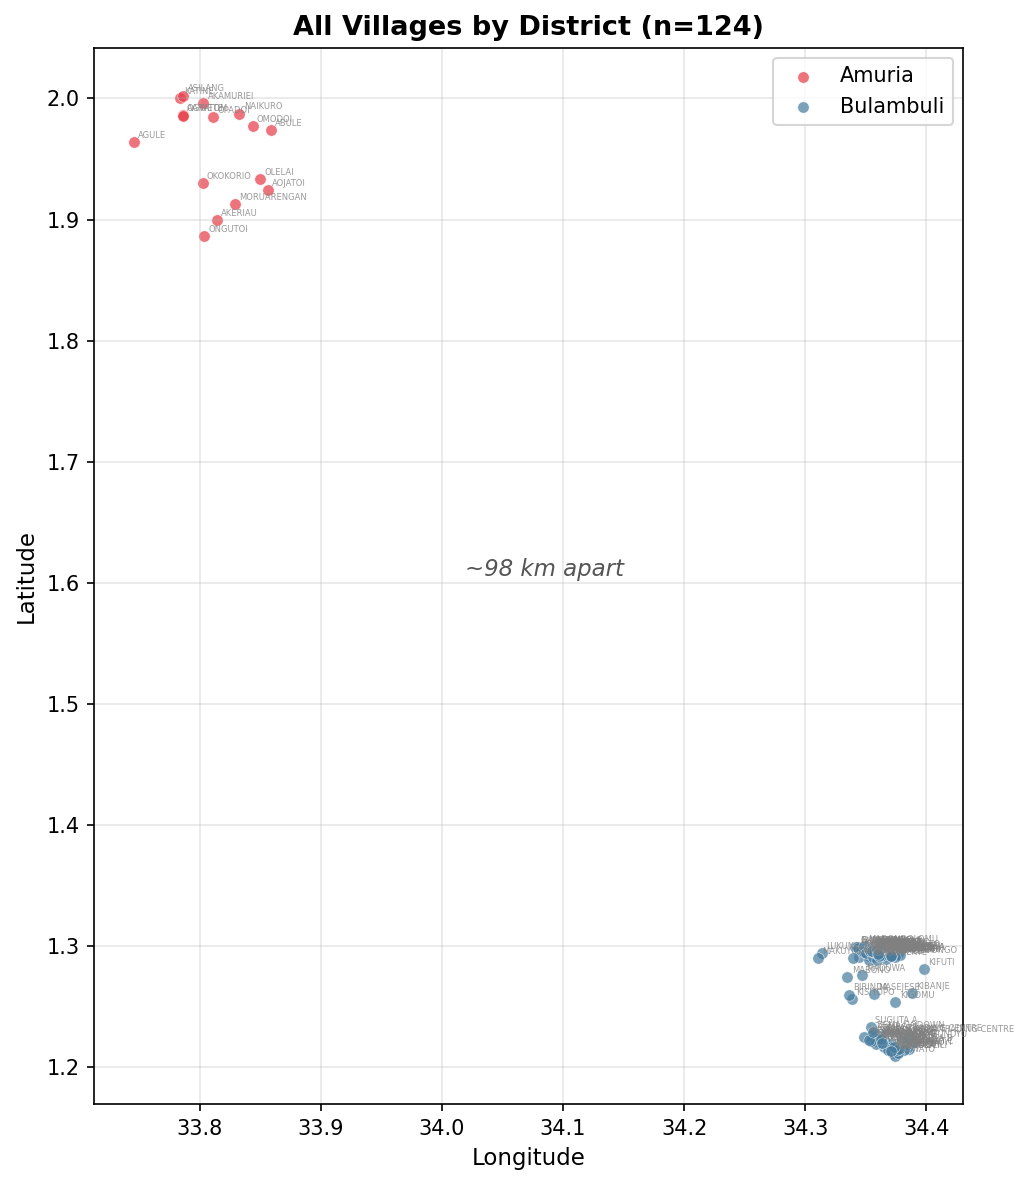
\includegraphics[width=0.95\textwidth]{figures/villages_all.png}
\caption{All study settlements by district. The two districts are approximately 98 km apart.}
\label{fig:villages_all}
\end{figure}

\begin{figure}[H]
\centering
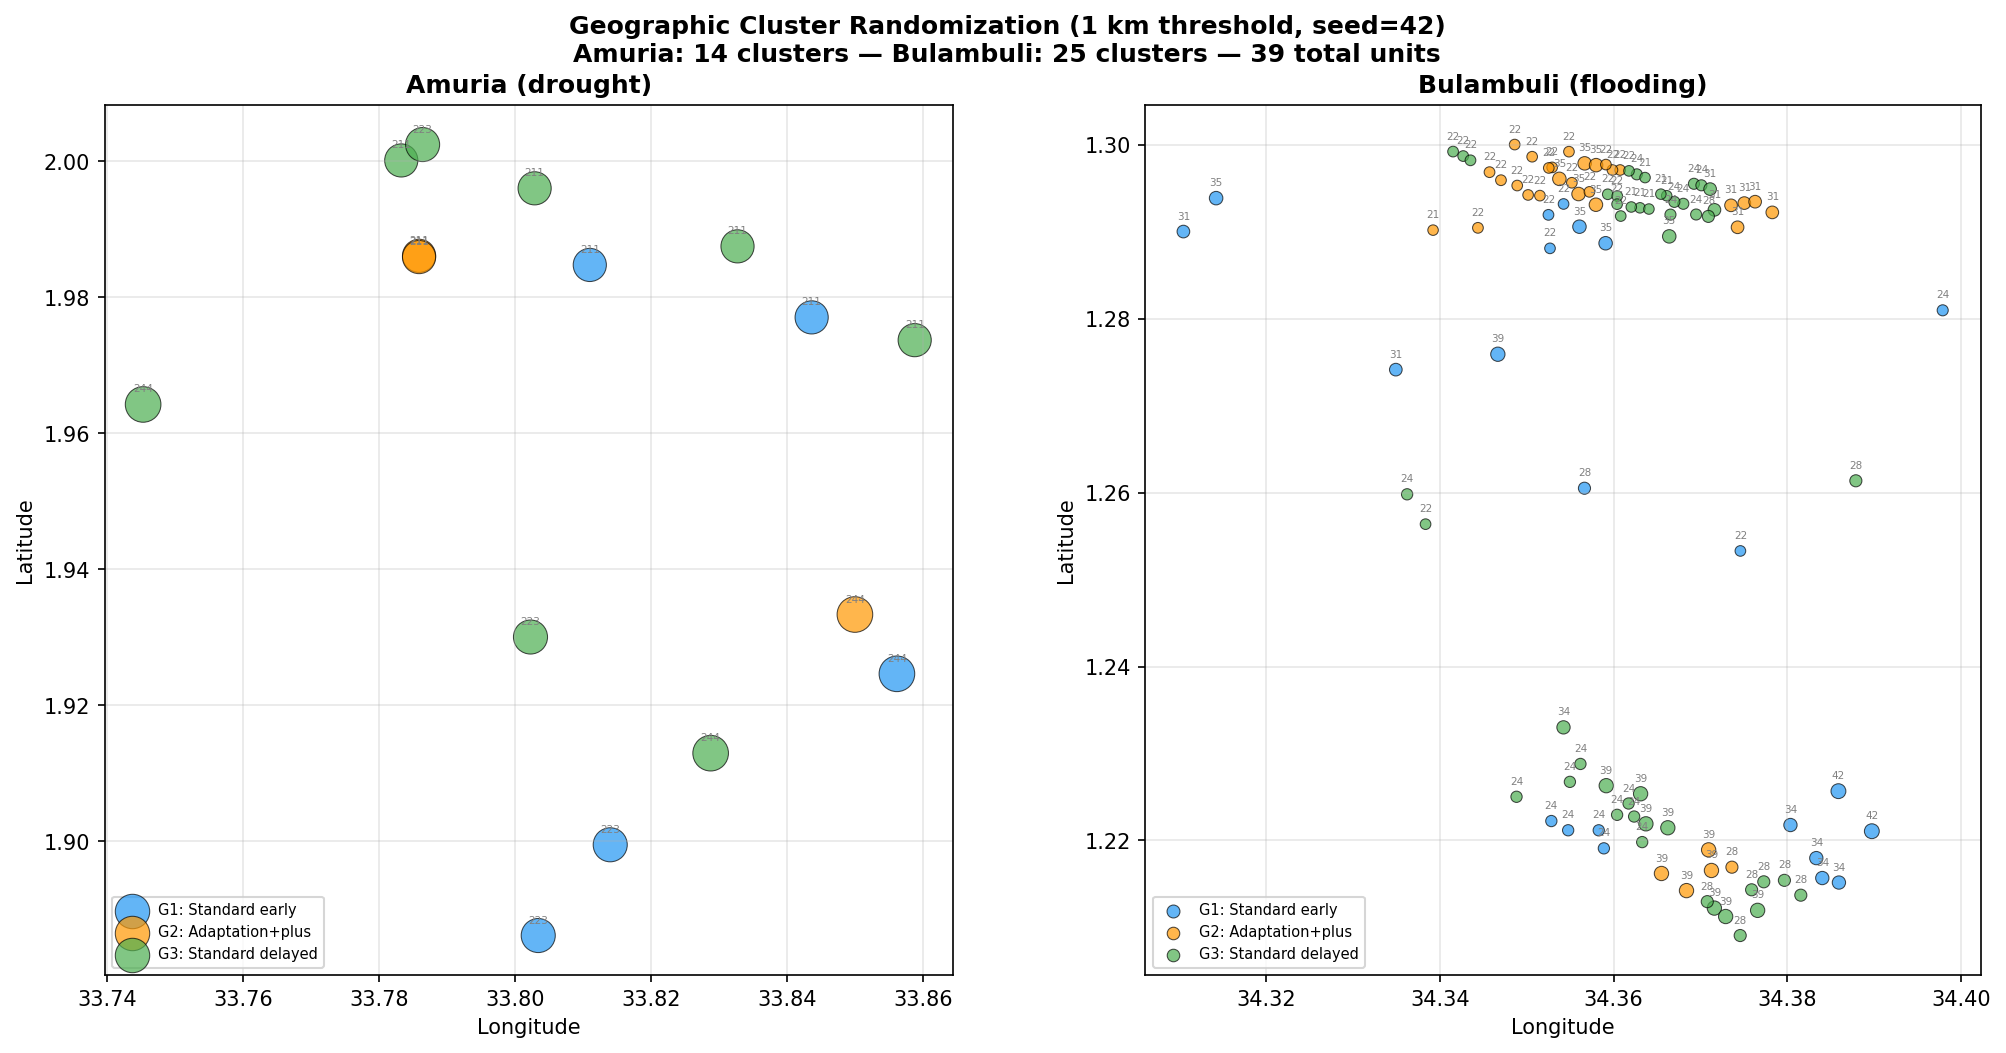
\includegraphics[width=0.95\textwidth]{figures/randomization_geo_1km.png}
\caption{Geographic cluster randomization at 1 km threshold.}
\label{fig:geo_1km}
\end{figure}

\begin{figure}[H]
\centering
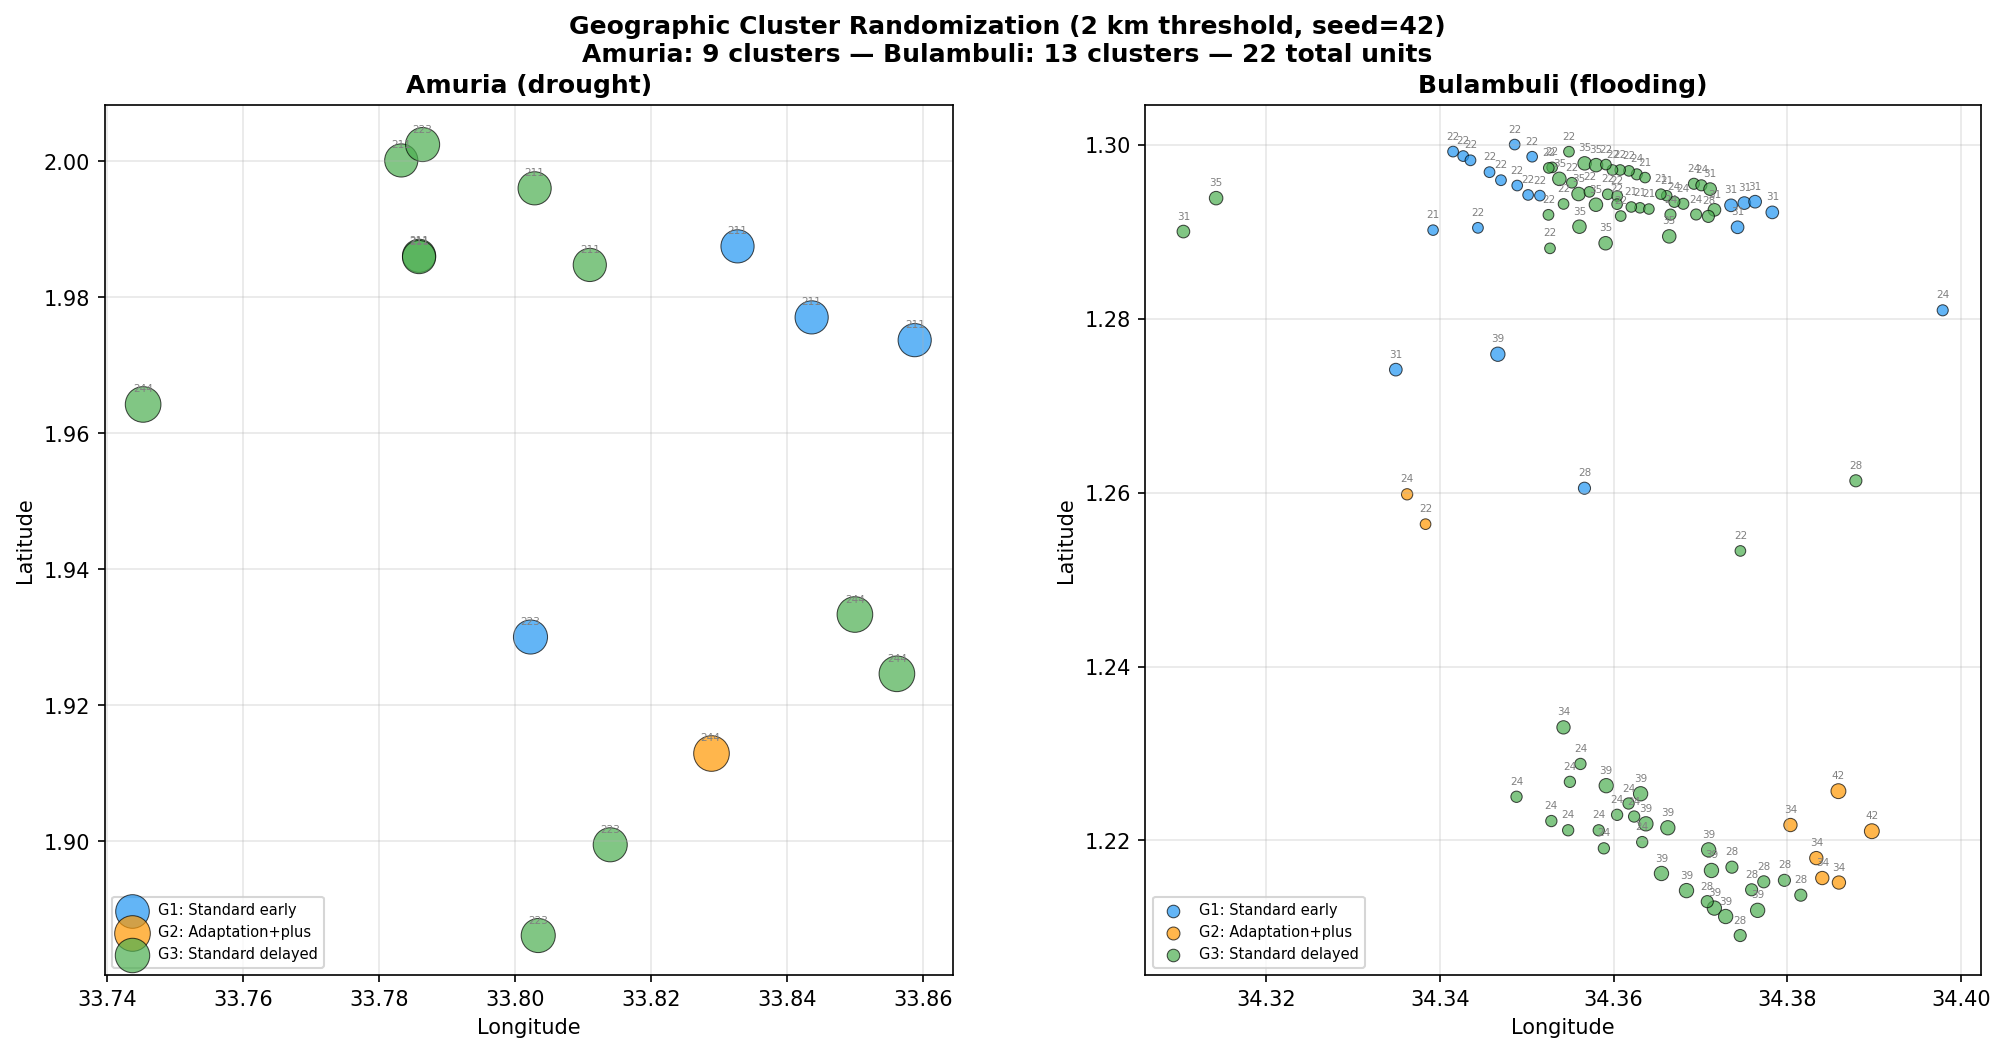
\includegraphics[width=0.95\textwidth]{figures/randomization_geo_2km.png}
\caption{Geographic cluster randomization at 2 km threshold.}
\label{fig:geo_2km}
\end{figure}

\begin{figure}[H]
\centering
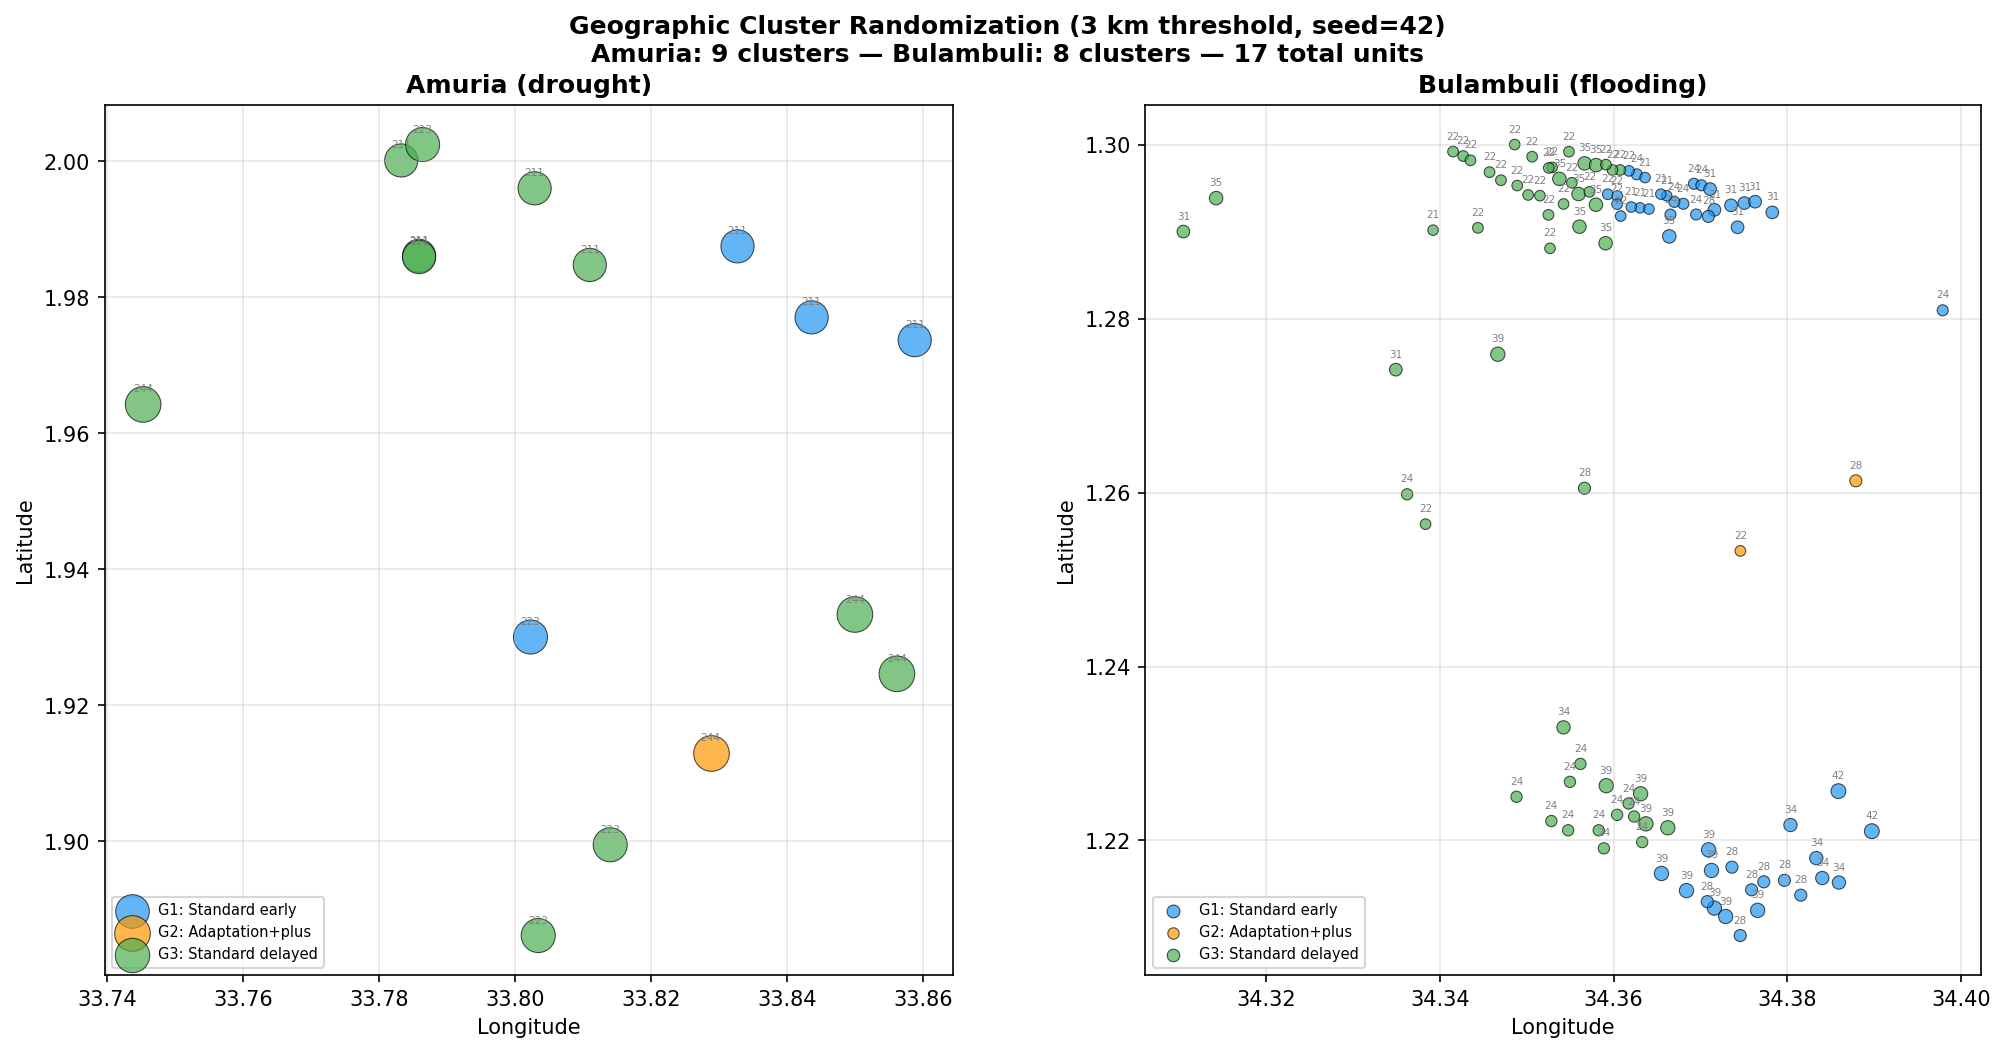
\includegraphics[width=0.95\textwidth]{figures/randomization_geo_3km.png}
\caption{Geographic cluster randomization at 3 km threshold.}
\label{fig:geo_3km}
\end{figure}

\begin{figure}[H]
\centering
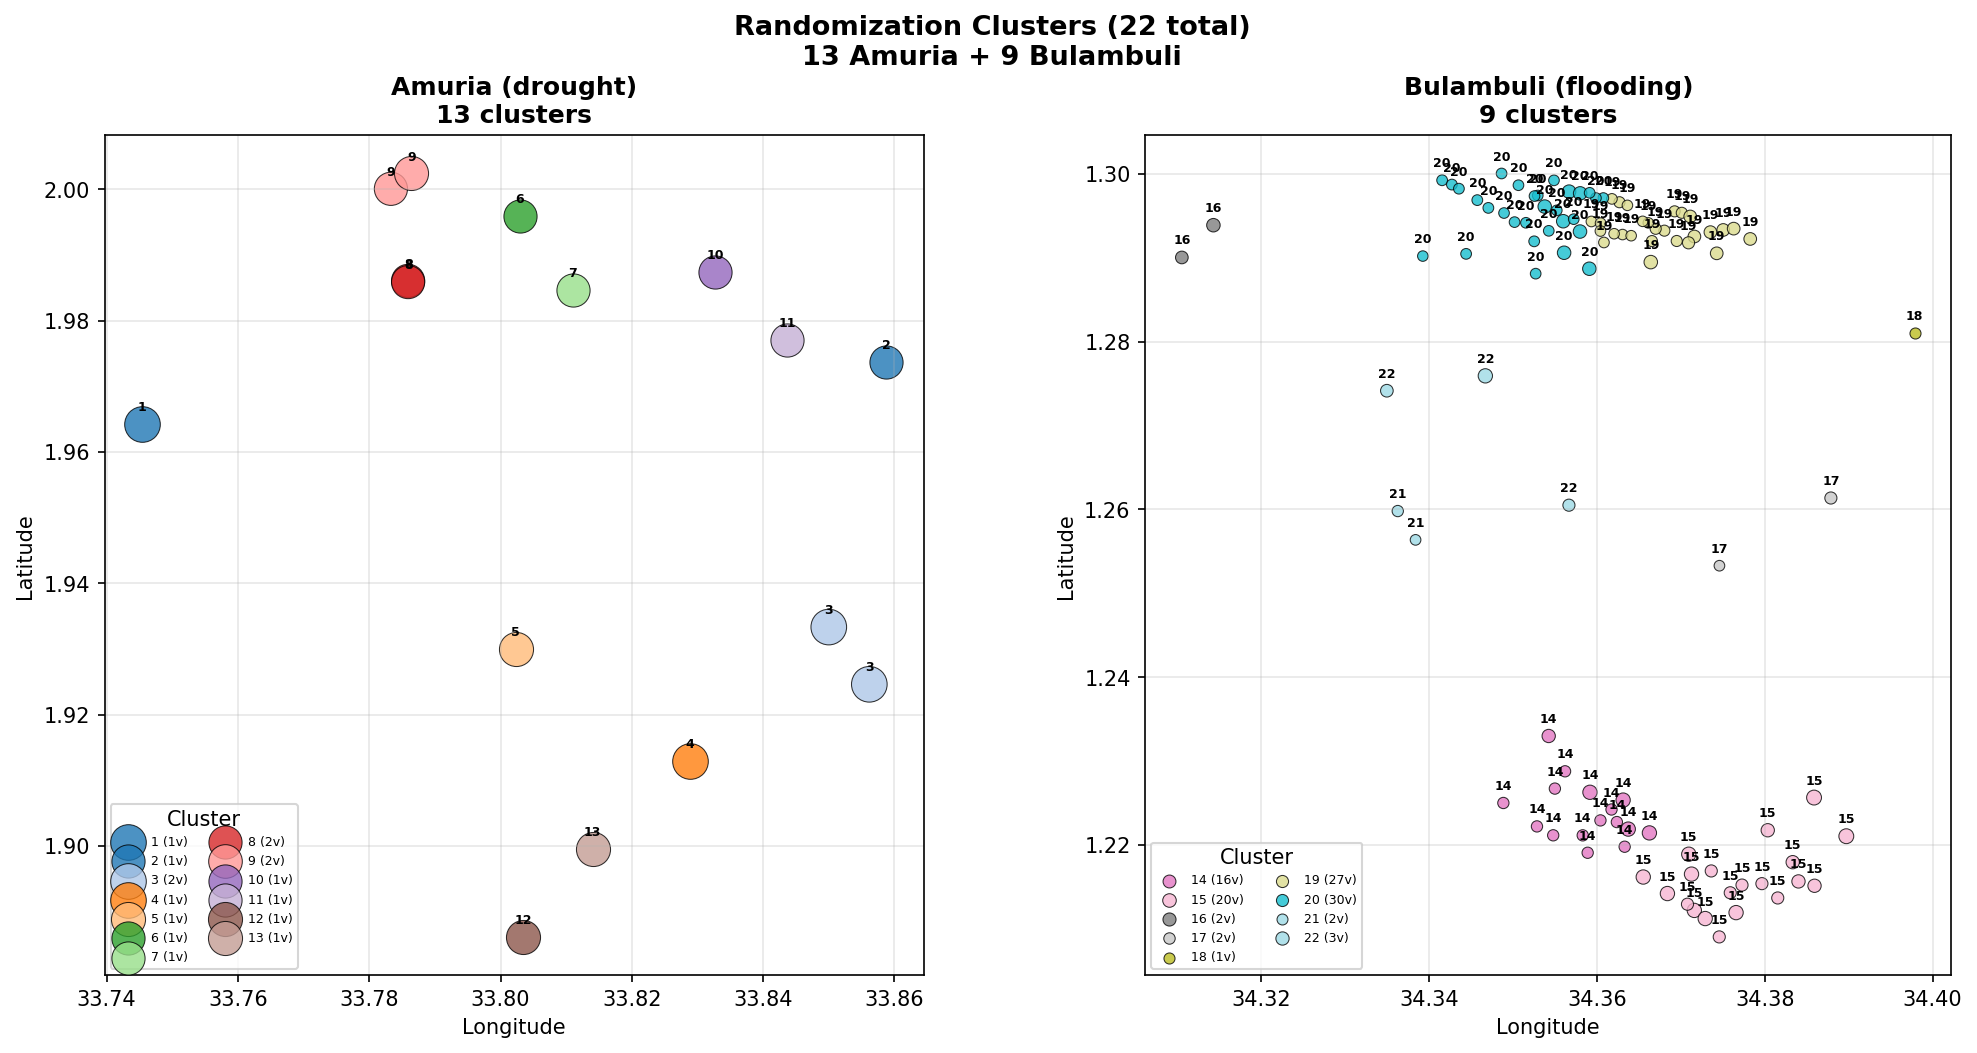
\includegraphics[width=0.95\textwidth]{figures/clusters_final_22.png}
\caption{Earlier cluster assignment at 3 km threshold with manual adjustments: 22 clusters (13 Amuria, 9 Bulambuli). Superseded by the 1 km automatic clustering (39 clusters).}
\label{fig:clusters_22}
\end{figure}

\bibliographystyle{apalike}
\bibliography{references}

\end{document}
